% !TEX root = ../main.tex
\chapter{Preliminaries}
\label{chap:preliminaries}

In this chapter I present the conceptual foundations and related technologies of my work. Also, I discuss the building blocks required to design a static analyzer framework for JavaScript.

\section{JavaScript}
Ohe most used dynamic languages in the world is JavaScript. According to~\cite{js-usage}, JavaScript is the most utilized client-side programming language for web applications, with over 94\% estimated usage. In this section I briefly summarize the history of JavaScript, present recent advancements and discuss why it is timely to utilize static analysis techniques for the language.

\subsection{From Glue Language to a Full-Fledged Language}
This section follows~\cite{10.1109/MC.2012.57}. The language written in 10 days by Brendan Eich in April 1995 --- originally called LiveScript --- was one of the first attempts at bringing dynamic behavior to the web. It was supposed to look like Java, leaving its complexity behind and appealing for developers looking for easy scripting solutions on the web.

The initial goal --- to create a language for portable applications --- has been seemingly achieved by the time of writing this report. While it has been gaining popularity due to its simpler syntax, the language, its tooling, and its community had time to evolve, making it the most used web programming language. JavaScript has shifted from simpler scripts to complex systems on the web, desktops, and servers.

\subsection{ECMAScript}
\label{sect:ecmascript}
After its release, JavaScript was submitted to and standardized by the Ecma International industry association, resulting in the first release of the ECMAScript language specification (of the ECMA-262 standard~\cite{ecma-262}) in June 1997. Apart from JavaScript, there are several implementations, e.g., \emph{ActionScript}, \emph{Chakra}, \emph{JScript}, and \emph{V8}.

There are several reasons why the standard and the usage of ECMAScript is getting more and more popular. Besides the improvement of the developer tools, developer community, and being already popular, conscious and regular development of the language also makes the language more appealing. At the time of writing this report there are 8 editions of the standard, 6 of them published. The last published edition, ES7 was published in June 2016, one year after the previous edition, ES6.

The initial language specifications were indulgent, and only best practices were guiding the developers. The challenges of analyzing such dynamic, untyped language --- able to express one thing in several different ways --- may be one of the reasons why there are only a few tools present even today implementing static analysis for ECMAScript.

The syntactic sugars added to the language across the editions of ECMAScript made it possible to express the most used code parts in an easier manner, while being more concise. Encouraging the developers to use these constructs makes it easier to interpret the source code --- both manually and with source code analysis.

% \subsection{Emerging Languages Translating to JavaScript}
% \subsubsection{WebAssembly}


\section{Static Analysis}
The idea of static analysis is almost half a century old. A paper from 1995 states that \textquote[\cite{wichmann_industrial_1995}]{The idea  that computer software should be used to analyze source programs rather than compile them, has a history of at least 25 years.}

Source code analysis can be used to discover facts about a particular program. Two basic automated analysis methods exist for this purpose:
\begin{itemize}[topsep=0pt]
  \item \emph{Static analysis} is performed by parsing the source code and analyzing it without evaluating the statements or executing the program.
  \item \emph{Dynamic analysis} is performed by executing the program and evaluating its output for given input sequences.
\end{itemize}

% > The term is usually applied to the analysis performed by an automated tool, with human analysis being called program understanding, program comprehension, or code review. Software inspections and Software walkthroughs are also used in the latter case.
% https://en.wikipedia.org/wiki/Static_program_analysis

While high-level language (e.g., C$++$, Java) source codes are checked at least by the compiler, JavaScript is usually not compiled before it is published. Thus a specific static analysis tool for JavaScript should aim to discover unwanted traits of the source in ways a generic compiler would not be able to, resulting in better code quality. These traits, \emph{code smells} are usually perceptible while running the code. Another way to locate these bugs is to write and run tests, dynamically testing the program.~\cite{wichmann_industrial_1995}

The two analysis methods are complementing each other. They discover different subsets of problematic constructions. While static analysis can discover syntactical problems (like the lack of the default case in a switch), dynamic analysis may catch behavioral problems (such as error handling and timing errors). Information discovered using static analysis may be used later in dynamic testing, resulting in a hybrid technique.

% > Static analysis bug-finding tools have evolved over the last several decades from basic syntactic checkers to those that find deep bugs by reasoning about the semantics of code. The goal of the Clang Static Analyzer is to provide a industrial-quality static analysis framework for analyzing C, C++, and Objective-C programs that is freely available, extensible, and has a high quality of implementation.
% http://clang-analyzer.llvm.org/


\subsection{Use Cases}
Static analysis tools employ diverse levels of abstraction. \emph{Formatters} are able to ensure that the source code complies with a predefined style guide. \emph{Linters} check for stylistic and programming errors, thus indicating suspicious programming constructs. \emph{Formal verification}, on the other hand, utilizes formal mathematical methods to prove statements about a piece of source code and its behavior.

For dynamic languages static analysis has even more use cases. For example, it allows finding previously undefined property reads, catching invocation of non-functional variables~\cite{jensen_type_2009}, detecting dead code.

\subsection{Advantages and Disadvantages}
Since static analysis tools deliberately do not evaluate the source code, there are fundamental limitations to what problems they can discover. In the context of my work, static analysis has the following trade-offs.

\subsubsection{Advantages}
\paragraph{No Need for Execution}
Since there is no need for execution, the hardware and software requirements of the analysis software do not need to match the requirements of the application. There is also no need to emulate or mock its dependencies, making the analysis more portable and cost efficient.

\paragraph{Early Detection of Possible Errors}
Static analysis may catch problems even before the whole software is complete or even runnable, potentially allowing the developers to fix the problems earlier in the development process.~\cite{xie}

\paragraph{Thorough}
While dynamic testing executes the manually written or automatically generated test cases covering a portion of the source code, static analysis systematically explores every possible execution scenarios. Thus it may achieve higher coverage and detect more problems in the code.~\cite{xie}

\subsubsection{Disadvantages}
\paragraph{Speed} Static analysis trades CPU time and memory for better code quality. By design it may be multiple orders of magnitude slower than compilation. Its speed depends not only on the underlying data structure and algorithms, but also the level of analysis.~\cite{clang}
% TODO extend

However, with a given limitation of granularity (e.g., considering a single file as the unit of processing), in case of a source code modification, previous results can be reused. There is a possibility that only the modified --- and other affected --- parts need to be processed again. The incremental approach of static analysis may speed up the process by orders of magnitude~\cite{stein-daniel-bsc}.
% TODO clarify

\paragraph{False Positives} Static analysis can not prove the correctness of a source code. It rather warns in case there is a possibility of a problem. Thus static analysis tools can introduce false positive warnings and flag code parts as problematic even if they behave correctly. To reduce the number of false positive warnings, one usually introduces more precise, specified rules and more thorough analysis.~\cite{clang}

\subsection{Source Code Processing and Analysis}
\label{sect:source-code-processing}
The source code of a program is a sequence of instructions formulated in a programming language as a text. Grammars of formal languages are a set of rules describing what the compiler considers a valid input---how to create valid instructions or a set of instructions from the alphabet of the language \emph{(syntax)}. A source code processing entity (transformer, or hereafter \emph{compiler}) assigns a meaning \emph{(semantics)} and transforms the instruction to another language (generally an intermediate language or bytecode).~\cite{Aho:1986:CPT:6448}

What input data the compiler considers useful information depends on the semantics of the language the compiler is built for. Source codes contain a much wider variety of data than a compiler requires for transforming, analyzing the application: comments, function declaration order, indentation, line breaks all help the reader (and writer) of the code, but carry no additional information.

\Cref{fig:processing-the-source-code} shows the general process for processing source code and transforming a stream of characters into a data structure with \emph{meaning} (semantic information).

\begin{figure}[!ht]
	\centering
	\adjustbox{max width=\textwidth} {
		\begin{tikzpicture}[
			node distance = 1cm,
      label distance = 0.5cm,
			auto,
			]

    \node[stdstage] (SC) {Source Code};
    \node[processor,
          below=of SC,
          label={left:tokenizer}
          ] (TOK) {};
    \node[stdstage, below=of TOK] (TO) {Tokens};
    \node[processor,
          below=of TO,
          label={left:parser}
          ] (PAR) {};
    \node[stdstage, below=of PAR] (AST) {Abstract Syntax Tree};
    \node[processor,
          below=of AST,
          label={left:scope analyzer}
          ] (SA) {};
    \node[stdstage, below=of SA] (ASG) {Abstract Semantic Graph};


    \path (SC) edge[flowedge]  (TOK);
    \path (TOK) edge[flowedge] (TO);
    \path (SC) edge[textedge] node {\emph{tokenization}\\ breaking the stream of source code characters into tokens (words, symbols)} (TO);

    \path (TO) edge[flowedge]  (PAR);
    \path (PAR) edge[flowedge] (AST);
    \path (TO) edge[textedge] node {\emph{parsing}\\ ordering the tokens into a data structure based on grammar rules} (AST);

    \path (AST) edge[flowedge]  (SA);
    \path (SA) edge[flowedge] (ASG);
    \path (AST) edge[textedge] node {\emph{scope analysis}\\ resolving the references in the AST and extending it with derived information into an ASG} (ASG);
		\end{tikzpicture}
	}
	\caption{Processing the source code.}
	\label{fig:processing-the-source-code}
\end{figure}

\subsubsection{Lexical Analysis}
A \emph{lexer}, \emph{tokenizer}, or \emph{scanner} forms the first phase of a parsing process. It scans the input character stream and segments them into sequence of groups, tokens, \emph{strings with a ``meaning''}. It also categorizes these groups into various token classes, token types. Processing the raw input into a value (converting the string \code{"2"} into the number $2$) can also happen in this phase. \Cref{fig:tokenization} shows how an expression string can be tokenized.

\begin{figure}[!htb]
  \centering
  \code{foo = 1 / 0}\\[1em]

  \begin{tabular}{c|l}
    Token & Token type\\
    \hline
    \code{foo} & \code{IDENTIFIER (Ident)}\\
    \code{=} & \code{ASSIGN (Punctuator)}\\
    \code{1} & \code{NUMBER (NumericLiteral)}\\
    \code{/} & \code{DIV (Punctuator)}\\
    \code{0} & \code{NUMBER (NumericLiteral)}\\
    \hline
  \end{tabular}

  \caption{Character stream and tokenization result with token type information.}
  \label{fig:tokenization}
\end{figure}


\subsubsection{Parser}
A \emph{parser} forms the second phase of a parsing process, using the output token stream of the \emph{lexer}. It takes the input data and builds a hierarchical data structure (a \emph{parse tree} or an \emph{abstract syntax tree}) representing the input. If the input does not comply with the syntax rules, and a tree can not be built, the source code is syntactically incorrect.

\Cref{fig:sentence-s-expression} shows a sentence and its s-expression representation. S-expressions (for ``symbolic expression'') are a notation for tree-structured nested list, mainly used in Lisp.

\begin{figure}[!htb]
\centering
\code{The quick brown fox jumps over the lazy dog}\\[1em]

\begin{minipage}{3cm}
\begin{verbatim}
(Sentence
  (Word The)
  (Word quick)
  (Word fox)
  (Word jumps)
  (Word over)
  (Word the)
  (Word lazy)
  (Word dog)
)
\end{verbatim}
\end{minipage}
  \caption{A sentence and its s-expression representation.}
  \label{fig:sentence-s-expression}
\end{figure}

\paragraph{Abstract Syntax Tree}
An \emph{Abstract Syntax Tree} (AST) is a tree representation of the syntactic structure of the result of a parsing along a grammar. The nodes of the tree denote a construct occurring in the input, while the edges represent the connection between these nodes based on the grammar rules.

As mentioned in~\cref{sect:source-code-processing}, source code contains much more detail (e.g., indentation, whitespace, comments) than is required and restrained during the parsing process. Thus this representation is a more compact, \emph{abstract} syntax tree. It may be transformed based on transformation rules and source code can be generated from ASTs. Without restraining the layout information and reusing it during the code generation, the resulting text can show differences in indents, whitespaces and expression formulation compared to the initial source code.

\Cref{fig:ast-asg-example} shows an example AST (in black), where a one-statement JavaScript file is parsed. The content of the file was only the following line:

\lstinputlisting[
  language=JavaScript
]{include/sources/oneliner.js}

\subsubsection{Scope Analyzer}
A \emph{scope analyzer} or \emph{context analyzer} produces a data structure that represents the scoping information of a program, extending the information available from an AST or an ASG. An element representing a scope in this data structure may contain, inter alia, metadata about the scope itself, the AST node related to the scope, available assets (variables, functions, etc.) in that scope.~\cite{shift-scope}

\paragraph{Abstract Semantic Graph}
An \emph{Abstract Semantic Graph} (ASG) differs from an Abstract Syntax Tree in two essential concepts: ASGs 1)~are not necessarily trees, and 2)~express more than the syntactic information; ASGs carry semantic information expressed with additional edges. An example of this type of edge connects variable references to their declarations.~\cite{raghavan_dex:_2004}

An ASG is a graph representation of a parse result; the nodes represent subterms of an expression. Shared subterms can occur, having more than one node linked to the same, common subterm. Compilers generally work on ASGs internally, since not only the syntactical, but the behavioral information is also represented in them.

% An abstract semantic graph is typically constructed from an abstract syntax tree by a process of enrichment and abstraction. The enrichment can for example be the addition of back-pointers, edges from an identifier node (where a variable is being used) to a node representing the declaration of that variable. The abstraction can entail the removal of details which are relevant only in parsing, not for semantics.
% https://en.wikipedia.org/wiki/Abstract_semantic_graph

\Cref{fig:ast-asg-example} shows the difference between an AST and an ASG (in turquoise).

\begin{figure}[!htb]
	\centering
	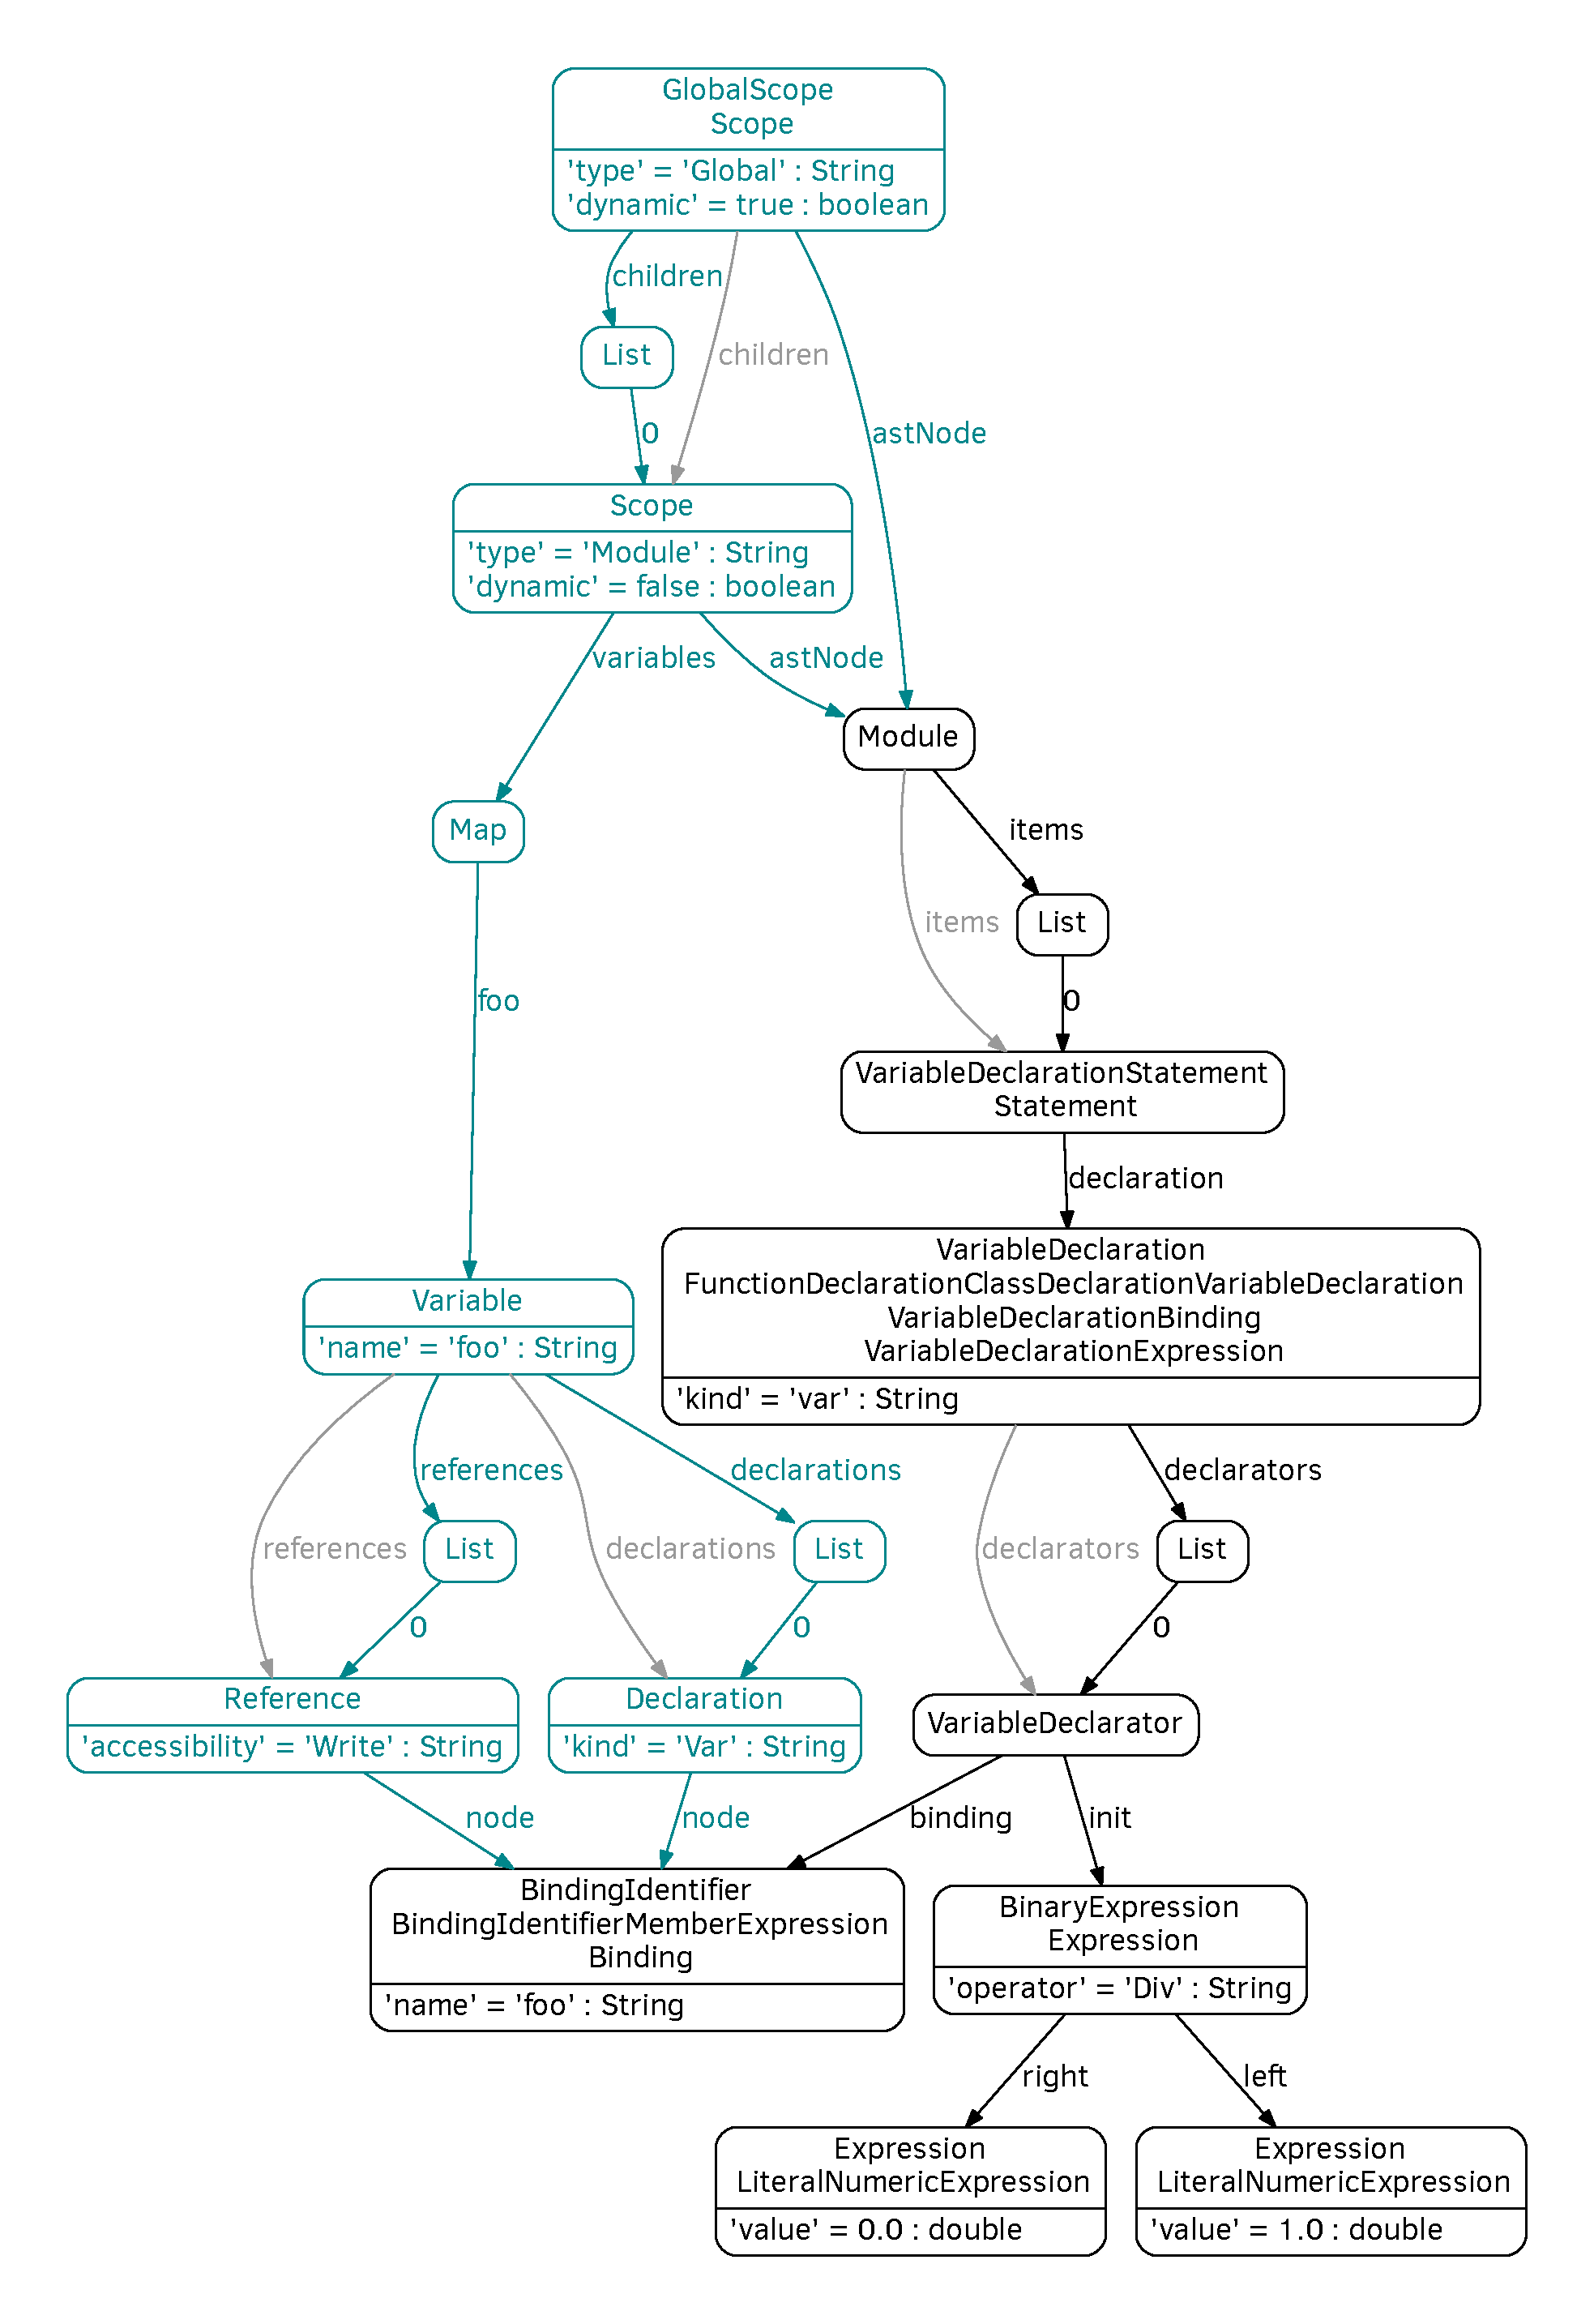
\includegraphics[height=\textheight, trim=1cm 1cm 1cm 1cm,clip]{include/figures/AST-ASG}
	\caption{AST (in black) with additional edges (ASG, in turquoise) and derived helper edges (in gray).}
	\label{fig:ast-asg-example}
\end{figure}

\FloatBarrier

%\section{Type Inference}
%
%Type inference refers to the deduction of the data types of expressions, statements during static analysis.
%
%> Type inference refers to the automatic deduction of the data type of an expression in a programming language. If some, but not all, type annotations are already present it is referred to as type reconstruction[citation needed]. The reverse operation of type inference is called type erasure.
%
%> It is a feature present in some strongly statically typed languages. It is often characteristic of functional programming languages in general. Some languages that include type inference are Nim, ML, OCaml, F\#, Haskell, Scala, Go, D, Clean, Opa, Rust, Swift, Visual Basic (starting with version 9.0), C\# (starting with version 3.0) and C++11. The ability to infer types automatically makes many programming tasks easier, leaving the programmer free to omit type annotations while still permitting type checking.
%
%% https://en.wikipedia.org/wiki/Type_inference
%
%\subsection{Typed JavaScript Derivations}
%
%\subsection{Analysis of JavaScript Source Codes}
%There are several static analysis frameworks and solutions available for JavaScript. I introduce and compare them in detail in \cref{sect:javascript-parsers} (JavaScript parsers) and \cref{sect:javascript-type-inferencers} (JavaScript type inferencing solutions).


\section{Handling Large Interconnected Data}
In numerous use cases, interconnected data sets can be represented and processed as a graph. \emph{Graph databases} provide a way to efficiently store graphs and evaluate graph queries. In this section I introduce the concept of graph databases, and graph pattern matching. I also present different types of graph database implementations from which I selected the most appropriate technology for the approach.

The advancements in hardware components -- the ever increasing amount of processing power, and memory and storage speed and sizes -- and the analogous growth of data to be stored and processed during the last more than fifty years yielded various solutions.

Based on historic evolution, these solutions can be categorized in three main categories:
\begin{itemize}[topsep=0pt]
  \item \emph{Navigational} database management systems (DBMS) were mainly used in the era of magnetic tape based storages, in which the \emph{records} contained references to other records allowing the system to fast-forward, \emph{navigate} there and load additional data.

  \item \emph{Relational} DBMSs organizes data in a \emph{relational model}~\cite{codd}, where one or more \emph{relations} contain unique entries (\emph{records} or \emph{tuples}).

  Relational databases leverage precise mathematical background (see \emph{relational algebra} and \emph{relational calculus}), have diverse implementations, mature tooling, and data access security by authentication and authorization. There are also disadvantages; due to their data structure, relational databases may have scalability and performance issues. They are also typically optimized for transactional processing and not data analysis (there are exceptions, see \emph{data warehouses}).

  \item \emph{Post-relational} databases is a vague collective name for every database system that abandons the strictness and burden of the relational data model and the Structured Query Language (SQL).

  Since the turn of the millennium, the struggle with storing and processing huge amounts of data using relational technologies spawned a diverse palette of new database management systems using simpler, more scalable data models. These systems are consequently called \emph{non SQL}, NoSQL databases, and are increasingly used in real-time and big data applications.

  NoSQL systems are a heterogeneous set of systems, with very different approaches. Categories of these systems based on their data models include, but are not limited to: \emph{key-value stores}, \emph{wide column stores}, \emph{document stores}, \emph{graph DBMSs}, \emph{RDF stores}.
\end{itemize}

\subsection{On Graph Computing}
The mathematical concepts of graphs are well-known and widely used in computer sciences. Numerous graph technologies have evolved, each with their advantages and disadvantages. From graphs themselves to physical and virtual worlds, many scenarios can be represented as graphs and stored in graph databases with their respective data model. This section loosely follows~\cite{scm, On_Graph_Computing}.
% TODO cite http://link.springer.com/article/10.1007%2Fs10586-015-0472-6

Simple, \emph{textbook-style} graphs can be extended in several different ways. To describe the connections in more detail, one may add directionality to edges (\emph{directed graph}). To allow different connections, one may label the edges (\emph{labeled graph}). \emph{Typed graphs} introduce types for vertices. \emph{Property graphs} add even more possibilities by introducing properties. Each graph element, both vertices and edges can be described with a collection of properties. The properties are key--value pairs, e.g.\ \texttt{type = `Person'}, \texttt{name = `John'}, \texttt{age = 34}.


\begin{figure}[htbp]
	\centering
	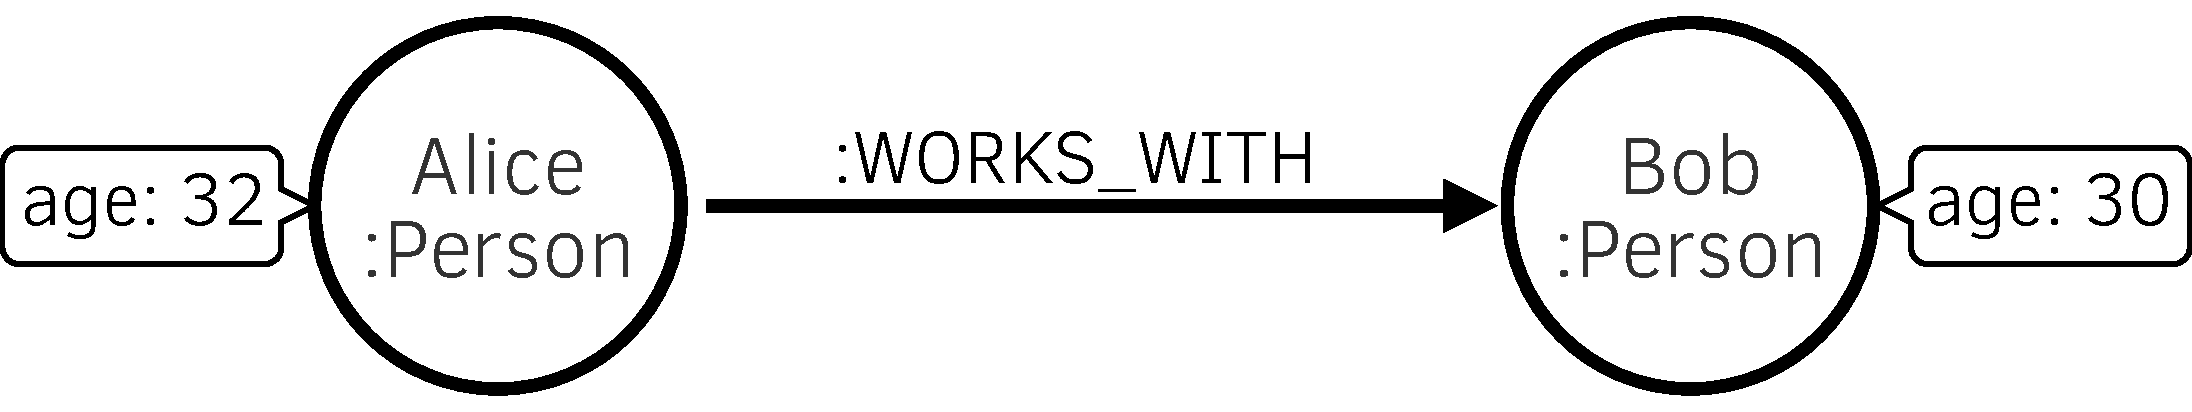
\includegraphics[width=0.6\textwidth]{graph-example}
	\caption{Typed and labeled property graph example.}
	\label{fig:graph-example}
\end{figure}


My approach utilizes typed (labeled) property graphs (see~\Cref{fig:graph-example}).

\subsubsection{Graph Computing Technologies}
The practice of data storage and processing is encumbered with space and time trade-off. This trade-off is also present in various graph computing technologies. This section discusses the categorization of these technologies and mentions a few technologies of which the most popular ones are detailed in~\cref{sect:graph-databases}.

The landscape of graph storing and processing solutions is populated and diverse (see~\cite{zhang_-memory_2015}). The basic categorization of software graph database solutions is the following. Graph computing technologies can be divided into two groups: 1)~on-line, real-time, and 2)~global analyzing, batch-processing graph databases. The former can be divided into in-memory, and persistent databases.

\paragraph{In-Memory Graph Toolkits}
The challenge of big data problems shed light on that the existing disk-based systems can not offer timely response due to the latency of hard disks. The role of storage shifted from the hard drive to the memory of the system. In-memory graph databases are constrained to graphs that fit into the main memory. Thus these systems are single-user systems that are oriented towards low-latency graph analysis.

The locality of data allows the usage of rich algorithm libraries and the choice of the adequate graph representation with respective space-time trade-off. The constraint of space allows large graphs (with millions of edges) to be stored and processed, but this may not be sufficient in all cases.

Example in-memory graph toolkits: \emph{Apache Giraph}\footnote{\small\url{http://giraph.apache.org}}, \emph{Microsoft Graph Engine}\footnote{\small\url{https://www.graphengine.io}} (formerly \emph{Trinity}), \emph{Apache Spark GraphX}\footnote{\small\url{http://spark.apache.org/graphx/}}, \emph{WhiteDB}\footnote{\small\url{http://whitedb.org}}.

\paragraph{Persistent, Real-Time Graph Databases}
Persistent graph databases are the prevalent group of graph computing technologies. Unlike in-memory graph tools, graph databases persist data on hard drives, thus are able to store billions of edges on a single machine and distributed systems can handle hundreds of billions of edges. These databases can provide multi-user concurrency, transactional semantics and eventual consistency.

Since global graph algorithms are not feasible, these systems are optimized for local neighborhood analysis and concurrent access. Global graph analytics are inefficient due to the communication overhead and the computational overhead, e.g., ensuring ACID transactional semantics.

Example for persistent, real-time graph databases: \emph{InfiniteGraph}\footnote{\small\url{http://www.objectivity.com/products/infinitegraph/}}, \emph{Neo4j} (see \cref{sect:neo4j}), \emph{OrientDB}\footnote{\small\url{http://orientdb.com}}, and \emph{Titan}~\cite{titan}.

\paragraph{Batch-Processing Graph Frameworks}
In case there is no real-time requirement for an analysis that accesses the whole dataset, batch-processing graph frameworks can be used for global analytics. Since there is also no requirement for quick response time, the applied algorithm can even scan data multiple times and leverage sequential reads from the disk. These systems can be used to periodically process data and feed back the results into real-time graph databases. Most of these frameworks utilize Hadoop for storage (HDFS) and processing algorithms implemented using the MapReduce paradigm.

Example batch-processing graph frameworks: \emph{Apache Hama}\footnote{\small\url{https://hama.apache.org}} and \emph{Apache Giraph}\footnote{\small\url{http://giraph.apache.org}}.

\subsection{Evaluating Queries on a Data Structure}
Numerous strategies exist for defining and executing queries over data structures. They can be defined in an imperative manner with programming languages like a navigation described in \emph{Gremlin}\footnote{\small\url{http://gremlin.tinkerpop.com}} over a graph database. Declarative solutions also exist, where the query plan is calculated from the query formalized in a declarative language (like \emph{SQL}\footnote{Structured Query Language}, \emph{SPARQL}\footnote{SPARQL Protocol and RDF Query Language}, and \emph{Cypher}) and execution is performed by a query framework (such as \emph{4store}\footnote{\small\url{https://github.com/garlik/4store}} and \emph{Neo4j}). Graph pattern matching -- one of the declarative querying solutions, supplemented by imperative logic -- forms the foundation of my approach.

\subsubsection{Graph Pattern Matching}
\textquote[\cite{csmr}]{Graph patterns are a declarative, graph-like formalism representing a condition (or constraint) to be matched against instance model graphs. The formalism is useful for various purposes in model-driven development, such as defining model transformation rules or defining general purpose model queries including model validation constraints. A graph pattern consists of structural constraints prescribing the interconnection between nodes and edges of a given type.

A match of a pattern is a tuple of pattern parameters that fulfill all the following conditions:
\begin{enumerate}[topsep=0pt]
	\item have the same structure as the pattern,
	\item satisfy all structural and attribute constraints,
	\item and does not satisfy any negative application condition (NAC) describing cases when the original pattern does not hold.
\end{enumerate}}

% TODO figure

\subsection{Graph Databases}
\label{sect:graph-databases}
Since my approach is based on graph-based data handling, it is essential to employ the most suitable technique. Related to my approach suitable refers to having the following traits: being fast, flexible, versatile, and easy to use and deploy. In this section I give an overview on the most promising candidates and justify why I have chosen Neo4j as the foundation of my approach.

\subsubsection{Neo4j}
\label{sect:neo4j}
Neo4j is the most popular~\cite{db-engines-ranking} and most mature NoSQL graph database, developed by \emph{Neo Technology}. It is open-source, well-documented and continuously-developed. Neo4j is available in two editions: a free \emph{Community Edition} and a paid \emph{Enterprise Edition}.~\cite{neo4j}

\paragraph{Architecture}
It can be deployed two ways: in \emph{server mode} the database is started separately and listens for queries on its HTTP REST and Bolt interface; where in \emph{embedded mode} it runs in the same JVM as the only client application.

\paragraph{Data Model}
The graph model of Neo4j is an implementation of a labeled property graph. The relations are labeled and the nodes can hold multiple labels; the nodes and relations can both hold properties.

\paragraph{Sharding}
Although the \emph{Enterprise Edition} of Neo4j has a high availability solution and supports clustered replication and cache sharding, it does not support sharded data storage over a cluster of devices. This results in the advantage of low latency (clustering provides scale out capabilities for read), the ability to handle transactions with ACID (Atomicity, Consistency, Isolation, and Durability) semantics.~\cite{neo4j-product}

\paragraph{Query Language}
Neo4j provides two methods for data queries out-of-the-box: an object-oriented native Java API for graph navigation and Cypher, a graph pattern description and query language with declarative and imperative traits. Additional interfaces may be loaded as a plugin, like the imperative Gremlin query interface~\cite{neo4j-gremlin-plugin}.

One of Cypher's best features is the readability of its syntax (see~\Cref{sect:division-by-zero} for examples). It provides an intuitive way to describe patterns of nodes and relations in the graph and also connections between subpatterns using bound identifiers for nodes and relations. Cypher also manages the indexes and constraints of the graph database. Negative application conditions (NAC) can be also expressed, describing constraints that should not hold for the matches.

Other interesting and useful features of Cypher include:
\begin{itemize}[topsep=0pt]
  \item Transitive closure over a set of edge labels, with optional repetition binding.

%        It is worth noting that an arbitrary sequence of edge labels can not be set as a repeating subpattern on its own, but temporary edges can be utilized to emulate this behavior.
  \item Java procedures can be stored in the server as a plug-in and called from inside the queries. This way an arbitrary logic with multiple queries can be stored on the Neo4j server and executed with a Cypher query. This can solve cases where it is not possible to express the query in Cypher; ranging from duplicating a node (with parameters and labels) to inferring the metamodel (from the nodes and relations already in the database).
  \item Parameterized queries may be utilized for faster evaluation.
%  \item List predicates evaluating predicates for all/any/none or single one nodes of the path.
%  \item Iterating and unwinding\footnote{transforming into rows} a collection in the query.
%  \item Finding the shortest path.
%  \item Mathematical functions.
%  \item Query profiling.
\end{itemize}

\subsubsection{Alternative Graph Databases}
Although other database solutions, like Titan~\cite{titan} or OrientDB might serve as an alternative, the rapid development and feature set of Neo4j ruled them out as a candidate for my approach.

For rapidly changing, albeit smaller datasets, incremental querying using VIATRA~\cite{viatra} Query over EMF~\cite{EMF} models can be a solution. Since VIATRA stores the database in-memory, it is not suitable for my approach.


\section{Integrated Development Environment (IDE)}
\label{sect:IDE}
Apart from the continuous integration workflow, static analysis tools are usually employed by developers within the integrated development environment they use. In this section I introduce one of the many freely available IDEs, and detail how static analysis tools can be integrated with it.

\subsection{Visual Studio Code}
\label{sect:visual-studio-code}
Visual Studio Code~\cite{vscode} is Microsoft's take on a lightweight, yet powerful Integrated Developer Environment for modern programming languages. It is available for free for Windows, macOS and Linux. It comes with built-in support for JavaScript, TypeScript and has a growing ecosystem of extensions for other languages, theming, and developer support~\cite{vscode-extensions}.

Debugging is also made easy, as the editor can be attached to the running code and the developer can add break points, look at call stacks and evaluate statements with an interactive console. With the relatively small package, Git support comes built-in: reviewing changed lines, staging files, making commits can be made right in the IDE.

\subsubsection{IntelliSense}
Visual Studio Code's syntax highlighting and autocomplete system is called IntelliSense, that also provides better completion based on variable types, function definitions, and imported modules. IntelliSense provides syntactical features like \emph{format on type}, \emph{outlining}; and also language service features like \emph{peek}, \emph{go to definition}, \emph{find all references} and \emph{rename symbol}.

To make these smarter functions possible, JavaScript service relies upon the TypeScript language service to handle JavaScript source code. It uses the same type inference system as TypeScript to determine the type of a value. (It recognizes the \emph{``ES3-style''} class declaration.) Explicit JSDoc annotations can also be used, in case the type inference does not provide the desired type information. For major libraries it is also possible to download an import a type definition file.

\subsubsection{Extensions}
Visual Studio Code is built with extensions in mind. Extensions make it possible to add new languages, themes, debuggers, and to connect to additional services. The framework runs them in a separate process, ensuring they will not slow the editor down.

Every extension uses the same model to describe its contribution (how it is registered in the framework), activation (when it is loaded) and the same way to access the VS Code extension API. There are two special type of extensions: language servers and debuggers, which have their own additional protocols.

Extensions are the building blocks of VS Code. When activated, every extension runs in a shared host process, separate from the IDE. This ensures that the IDE itself can remain responsive even if an extension is resource-heavy or not well-written.

An extension is a package of source code, resources, and configuration files. They have support for:
\begin{itemize}[topsep=0pt]
  \item Activation -- it is possible to specify when an extension is loaded: when a specific file type exists in the workspace or is opened; or when a command (described in the configuration) is executed via the \emph{Command Palette} or the key combination.
  \item Editor -- the extension can read and manipulate the editor's content.
  \item Workspace -- the extension can access working files, modify the content of the status bar and show information messages (and more).
  \item Eventing -- it is also possible to subscribe and react to the life-cycle events of the editor such as: open, close, change events of the editor (and more).
  \item Evolved editing -- rich language support can be provided, including IntelliSense services, peek, hover and diagnostic (info, warning and error messages).
\end{itemize}

\paragraph{Language Servers} The language server framework and its sample implementation helps developers create a dedicated process for resource-heavy language server applications. It is the better design choice if the extension may slow down other extensions while working. Its possibilities are limited, as custom communication between the client extension and the language server needs modification in the underlying communication protocol handler.

\paragraph{Debuggers} Connecting an external debugger written for any language to VS Code is also possible through the VS Code Debug protocol.

\subsection{Alternative IDEs}
There are several alternatives to Visual Studio Code. \emph{Atom}\footnote{\small\url{https://atom.io}}, \emph{Eclipse}\footnote{\small\url{https://eclipse.org}}, and \emph{WebStorm}\footnote{\small\url{https://www.jetbrains.com/webstorm/}} can all be extended with a plugin adding extra features for a given language. Since VSC is one of the most actively developed lightweight IDEs aiming for JavaScript (and TypeScript) development, I have developed an extension integrating the IDE with my framework (see~\Cref{sect:ide-integration}).
